\documentclass[10pt]{article}
\usepackage[a4paper,margin=22mm]{geometry}
\usepackage{amsmath,booktabs,graphicx}
\usepackage[T1]{fontenc}
\usepackage{lmodern}
\setlength{\parindent}{0pt}
\setlength{\parskip}{5pt}

\begin{document}

\section*{HNL Construction Cost and Interaction-List Reuse}

This report evaluates the measured cost of the hierarchical neighborhood
layer (HNL) construction without comparing it with another traversal.  The
first study measures list construction and deterministic work counts on a
five-mesh adaptive sequence.  The second study measures the benefit of
retaining the same HNL--MAC interaction lists during a manufactured sequence
of density updates.  These experiments demonstrate practical behavior over
the tested range; they do not prove an asymptotic complexity bound.

\subsection*{Work growth under mesh refinement}

All cases use $(p,P,\theta)=(6,4,0.5)$ and 16 OpenMP threads.  Each timing is
the median of three runs performed in interleaved order.  The work counters
are deterministic, and every source-partition check passes.

\begin{table}[htbp]
\centering
\small
\setlength{\tabcolsep}{4.5pt}
\begin{tabular}{rrrrrrrr}
\toprule
$N$ & depth & $T_{\rm list}$ (s) & $\mu$s/target & candidates & materialization & MAC visits & list entries \\
\midrule
10\,328  & 4 & 0.124 & 12.00 & 463.3  & 506.6  & 1\,856.1 & 1\,679.8 \\
34\,464  & 5 & 0.678 & 19.68 & 775.6  & 860.5  & 2\,800.6 & 2\,545.1 \\
100\,656 & 5 & 1.957 & 19.44 & 769.9  & 856.0  & 2\,768.2 & 2\,516.2 \\
191\,544 & 5 & 5.284 & 27.59 & 1\,104.0 & 1\,234.9 & 3\,549.1 & 3\,240.9 \\
822\,720 & 6 & 24.152 & 29.36 & 1\,174.5 & 1\,317.4 & 3\,723.2 & 3\,402.3 \\
\bottomrule
\end{tabular}
\end{table}

The number of active leaves increases by a factor of 79.7.  Over the same
sequence, the average candidate, materialization, MAC-visit, and final-list
counts increase by factors of 2.54, 2.60, 2.01, and 2.03, respectively.
Thus the measured work per target grows moderately for this mesh family,
although the data do not establish a mesh-independent bound.

\subsection*{Repeated density updates}

The reuse study uses $N=100\,656$, $(p,P,\theta)=(6,4,0.5)$, and 64 OpenMP
threads.  At each step the control path rebuilds the same HNL--MAC lists,
whereas the reuse path retains the initial lists and updates only the density
samples, moments, and potential.  Every rebuilt list agrees exactly with its
cached counterpart.

\begin{table}[htbp]
\centering
\begin{tabular}{rrrrr}
\toprule
Updates & rebuild total (s) & reuse total (s) & saved (\%) & speedup \\
\midrule
1  & 2.798  & 2.950  & $-0.9$ & 0.991 \\
2  & 5.570  & 4.857  & 13.3 & 1.154 \\
5  & 13.684 & 10.612 & 22.5 & 1.290 \\
10 & 27.245 & 20.193 & 25.9 & 1.349 \\
20 & 53.934 & 38.988 & 27.6 & 1.381 \\
\bottomrule
\end{tabular}
\end{table}

After 20 updates, one-time construction followed by reuse reduces cumulative
time by 27.6\% and gives a 1.381-fold speedup.  The one-update case shows no
benefit because the one-time setup has not yet been amortized.  This is a
manufactured SCF-like sequence, not a Kohn--Sham SCF calculation.

\begin{figure}[htbp]
\centering
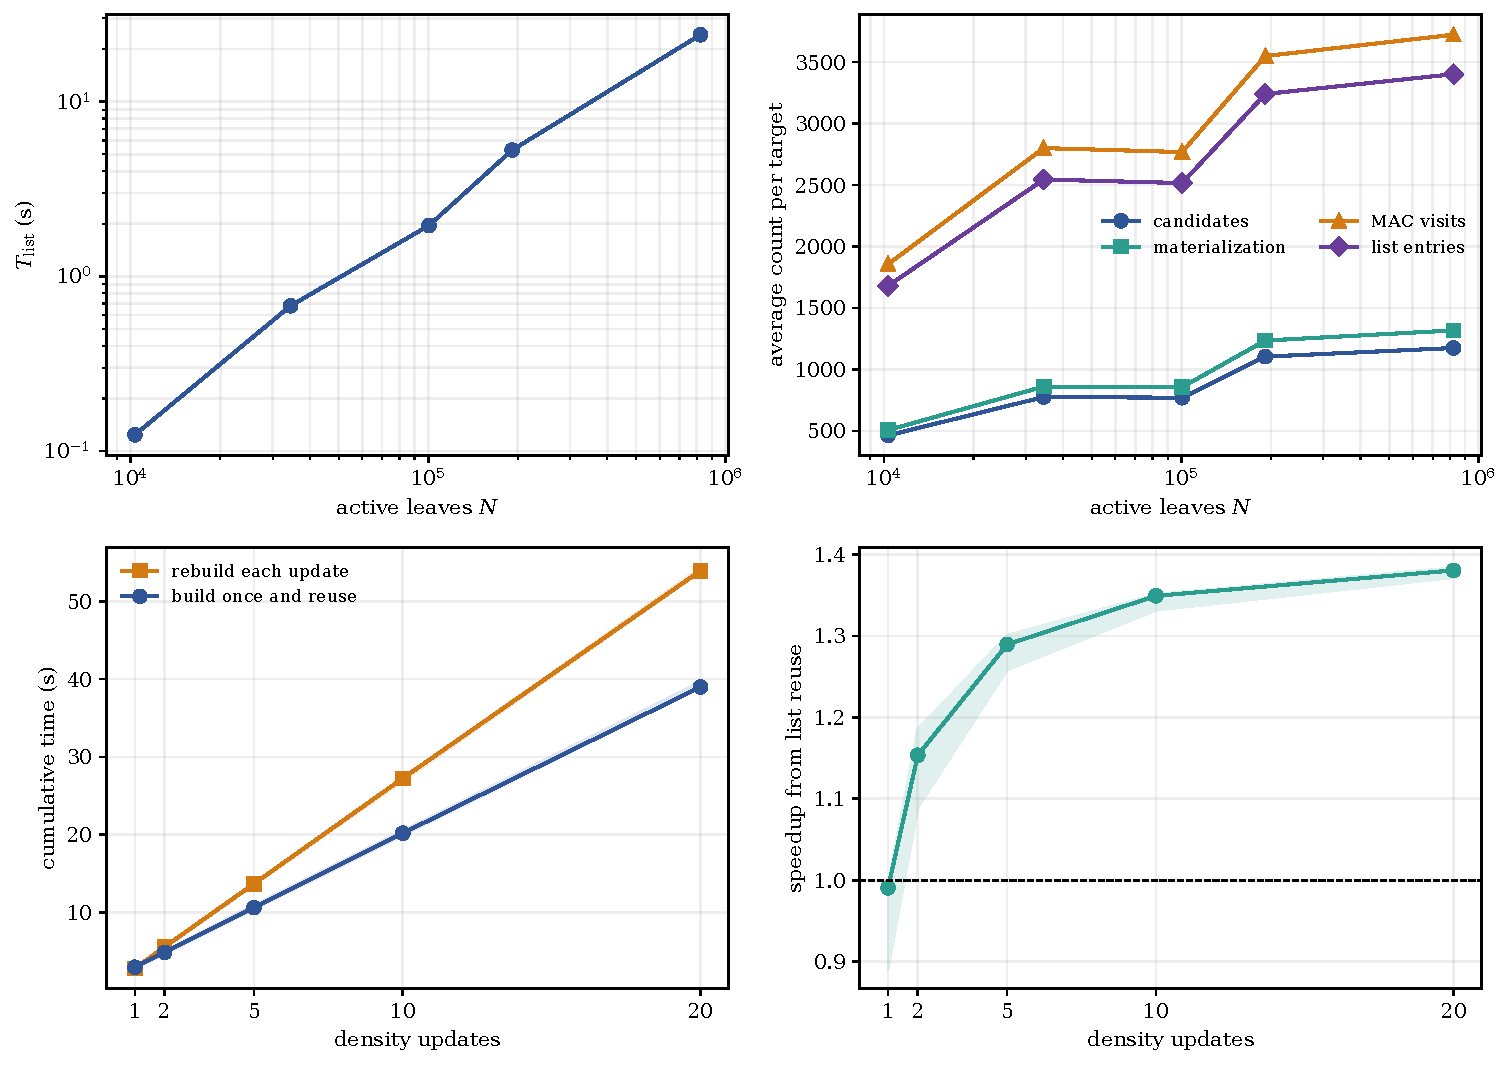
\includegraphics[width=\textwidth]{hnl_efficiency.pdf}
\caption{Measured HNL construction work (top) and repeated-density list reuse
(bottom).  Bands show the ranges over three runs.}
\end{figure}

The server load was nonzero during the runs, particularly in the 64-thread
reuse study.  The three repeats are close and the rebuild and reuse paths are
measured within the same runs, but publication-quality absolute timings
should be repeated on an otherwise idle machine.

\end{document}
